



%%%%%%%%%%%%%%%%%%%%%%%%%%%%%%%%%%%%%%%%%
% Beamer Presentation
% LaTeX Template
% Version 1.0 (10/11/12)
%
% This template has been downloaded from:
% http://www.LaTeXTemplates.com
%
% License:
% CC BY-NC-SA 3.0 (http://creativecommons.org/licenses/by-nc-sa/3.0/)
%
%%%%%%%%%%%%%%%%%%%%%%%%%%%%%%%%%%%%%%%%%

%----------------------------------------------------------------------------------------
%	PACKAGES AND THEMES
%----------------------------------------------------------------------------------------

\documentclass[aspectratio=169]{beamer}

\mode<presentation> {


% The Beamer class comes with a number of default slide themes
% which change the colors and layouts of slides. Below this is a list
% of all the themes, uncomment each in turn to see what they look like.

%\usetheme{default}
%\usetheme{AnnArbor}
%\usetheme{Antibes}
%\usetheme{Bergen}
%\usetheme{Berkeley}
%\usetheme{Berlin}
%\usetheme{Boadilla}
%\usetheme{CambridgeUS}
%\usetheme{Copenhagen}
%\usetheme{Darmstadt}
%\usetheme{Dresden}
%\usetheme{Frankfurt}
%\usetheme{Goettingen}
%\usetheme{Hannover}
%\usetheme{Ilmenau}
%\usetheme{JuanLesPins}
%\usetheme{Luebeck}
\usetheme{Madrid}
%\usetheme{Malmoe}
%\usetheme{Marburg}
%\usetheme{Montpellier}
%\usetheme{PaloAlto}
%\usetheme{Pittsburgh}
%\usetheme{Rochester}
%\usetheme{Singapore}
%\usetheme{Szeged}
%\usetheme{Warsaw}

% As well as themes, the Beamer class has a number of color themes
% for any slide theme. Uncomment each of these in turn to see how it
% changes the colors of your current slide theme.

%\usecolortheme{albatross}
%\usecolortheme{beaver}
%\usecolortheme{beetle}
%\usecolortheme{crane}
%\usecolortheme{dolphin}
%\usecolortheme{dove}
%\usecolortheme{fly}
%\usecolortheme{lily}
%\usecolortheme{orchid}
%\usecolortheme{rose}
%\usecolortheme{seagull}
%\usecolortheme{seahorse}
%\usecolortheme{whale}
%\usecolortheme{wolverine}

%\setbeamertemplate{footline} % To remove the footer line in all slides uncomment this line
%\setbeamertemplate{footline}[page number] % To replace the footer line in all slides with a simple slide count uncomment this line

\definecolor{UOSred}{rgb}{0.6745098039215686, 0.02352941176470588, 0.2039215686274510} % UBC Blue (primary)
\definecolor{UOSgrey}{rgb}{0.8117647058823529, 0.8117647058823529, 0.8117647058823529} % UBC Grey (secondary)

\setbeamercolor{palette primary}{bg=UOSred,fg=white}
\setbeamercolor{palette secondary}{bg=UOSred,fg=white}
\setbeamercolor{palette tertiary}{bg=UOSred,fg=white}
\setbeamercolor{palette quaternary}{bg=UOSred,fg=white}
\setbeamercolor{structure}{fg=UOSred} % itemize, enumerate, etc
\setbeamercolor{section in toc}{fg=UOSred} % TOC sections

%gets rid of bottom navigation bars
\setbeamertemplate{footline}[frame number]{}

%gets rid of bottom navigation symbols
\setbeamertemplate{navigation symbols}{}


\usepackage{amsmath}
\usepackage{selinput}      % Halbautomatische Auswahl der Eingabecodierung
\SelectInputMappings{      % mit Hilfe ausgewählter Glyphen
  adieresis={ä},	   % siehe: http://partners.adobe.com/public/developer/en/opentype/glyphlist.txt
  germandbls={ß},
  Euro={€}
}

\addtobeamertemplate{footline}{%
  \leavevmode%
  \hbox{%
  \begin{beamercolorbox}[wd=\paperwidth,ht=2.25ex,dp=1ex,center]{author in head/foot}%
     \insertsectionnavigationhorizontal{\paperwidth}{}{}
  \end{beamercolorbox}}%

}

% Override palette coloring with secondary
\setbeamercolor{subsection in head/foot}{bg=UOSgrey,fg=white}

%\setbeamertemplate{navigation symbols}{} % To remove the navigation symbols from the bottom of all slides uncomment this line
}
\usepackage{hyperref}
\usepackage{graphicx} % Allows including images
\usepackage{grffile}
\usepackage{booktabs} % Allows the use of \toprule, \midrule and \bottomrule in tables
\graphicspath{{images/}}
%----------------------------------------------------------------------------------------
%	TITLE PAGE
%----------------------------------------------------------------------------------------

\title[Übungsprojekt Phase 1]{Übungsprojekt Phase 1} % The short title appears at the bottom of every slide, the full title is only on the title page

\author{T. Adam, M. ben Ahmed} % Your name
\institute[UOS] % Your institution as it will appear on the bottom of every slide, may be shorthand to save space
{

Universität Osnabrück \\ % Your institution for the title page

\medskip
\textit{Æ} % Your email address


}
\date{\today} % Date, can be changed to a custom date

\begin{document}

\begin{frame}
\titlepage % Print the title page as the first slide
\end{frame}


%----------------------------------------------------------------------------------------
%	PRESENTATION SLIDES
%----------------------------------------------------------------------------------------


%------------------------------------------------

\begin{frame}
	\frametitle{(A) Benchmark-Instanzen}
	\begin{columns}[c] % The "c" option specifies centered vertical alignment while the "t" option is used for top vertical alignment
	
	\column{.5\textwidth} % Right column and width
	\begin{itemize}
		\item Welche Instanzen werden in der Literatur verwendet? \pause
		
	\end{itemize}
	
	\column{.45\textwidth} % Left column and width
	\begin{enumerate}
	\item Generiert: gleichverteilte Punkte\pause
	\item Generiert: Cluster mit umliegenden Punkten\pause
	\item Geografisch: Bahnhöfe, Städte, Sehenswürdigkeiten
	
	\end{enumerate}
	

	\end{columns}
	\end{frame}
%------------------------------------------------

\begin{frame}
	\frametitle{(A) Benchmark-Instanzen}
	\begin{columns}[c] % The "c" option specifies centered vertical alignment while the "t" option is used for top vertical alignment
	
	\column{.5\textwidth} % Right column and width
	\begin{itemize}
		\item Welche Eigenschaften machen eine Instanz interessant um Algorithmen darauf zu testen? \pause
	\end{itemize}
	
	\column{.45\textwidth} % Left column and width
	\textbf{Punktdichte}
	\begin{enumerate}

	\item Dicht genug, damit Label clever platziert werden müssen. \pause
	\item Nicht zu dicht, damit Label platziert werden können. 
	\end{enumerate}
	

	\end{columns}
	\end{frame}
%------------------------------------------------


\begin{frame}
	\frametitle{(A) Benchmark-Instanzen}
	\begin{columns}[c] % The "c" option specifies centered vertical alignment while the "t" option is used for top vertical alignment
	
	\column{.5\textwidth} % Right column and width
	\textbf{Generiert: Gleichverteilte Punkte}
	\begin{itemize}
		\item 100 Instanzen mit 100 - 10000 Punkten
	\end{itemize}
	
	\column{.45\textwidth} % Left column and width
	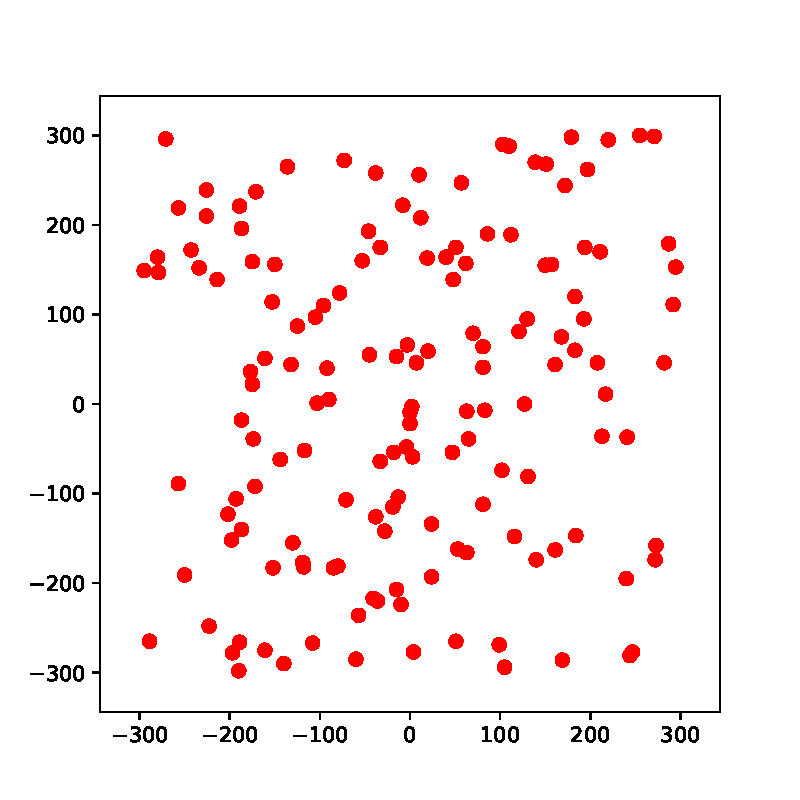
\includegraphics[scale=.5]{random.pdf}
	

	\end{columns}
	\end{frame}

%------------------------------------------------


\begin{frame}
	\frametitle{(A) Benchmark-Instanzen}
	\begin{columns}[c] % The "c" option specifies centered vertical alignment while the "t" option is used for top vertical alignment
	
	\column{.5\textwidth} % Right column and width
	\textbf{Generiert: Gleichverteilte Punkte}
	\begin{itemize}
		\item 100 Instanzen mit 100 - 10000 Punkten
	\end{itemize}
	
	\column{.45\textwidth} % Left column and width
	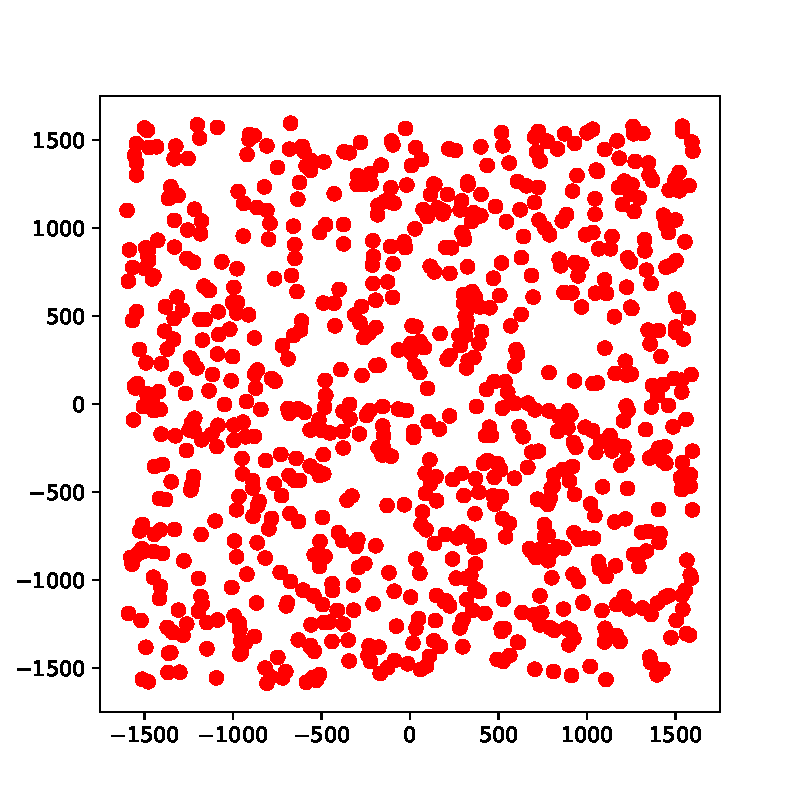
\includegraphics[scale=.5]{random_big.pdf}
	

	\end{columns}
	\end{frame}

%------------------------------------------------

\begin{frame}
	\frametitle{(A) Benchmark-Instanzen}
	\begin{columns}[c] % The "c" option specifies centered vertical alignment while the "t" option is used for top vertical alignment
	
	\column{.5\textwidth} % Right column and width
	\textbf{Generiert: Gleichverteilte Punkte}\\
	Erfolgsquote des primitiven Algorithmus
	
	
	\column{.45\textwidth} % Left column and width
	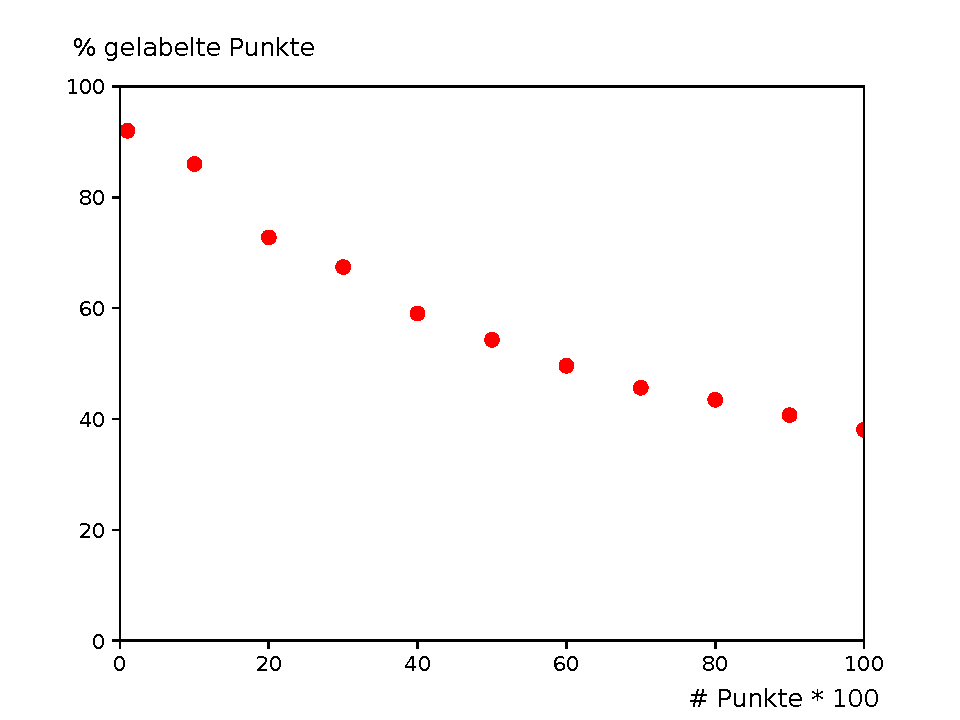
\includegraphics[scale=.45]{random_solve.pdf}
	

	\end{columns}
	\end{frame}

%------------------------------------------------



\begin{frame}
	\frametitle{(A) Benchmark-Instanzen}
	\begin{columns}[c] % The "c" option specifies centered vertical alignment while the "t" option is used for top vertical alignment
	
	\column{.5\textwidth} % Right column and width
	\textbf{Generiert: Cluster}
	\begin{itemize}
		\item 100 Instanzen mit 100 - 10000 Punkten
		\item Clusterzentren umgeben von weiteren Punkten
	\end{itemize}
	
	\column{.45\textwidth} % Left column and width
	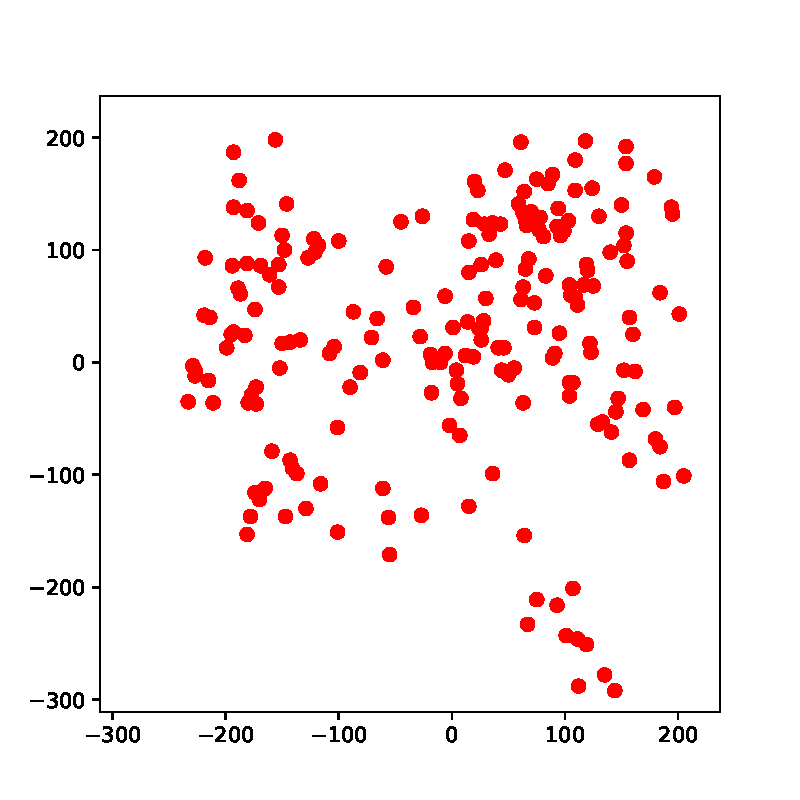
\includegraphics[scale=.5]{cluster.pdf}
	

	\end{columns}
	\end{frame}

%------------------------------------------------


\begin{frame}
	\frametitle{(A) Benchmark-Instanzen}
	\begin{columns}[c] % The "c" option specifies centered vertical alignment while the "t" option is used for top vertical alignment
	
	\column{.5\textwidth} % Right column and width
	\textbf{Generiert: Cluster}
	\begin{itemize}
		\item 100 Instanzen mit 100 - 10000 Punkten
		\item Clusterzentren umgeben von weiteren Punkten
	\end{itemize}
	
	\column{.45\textwidth} % Left column and width
	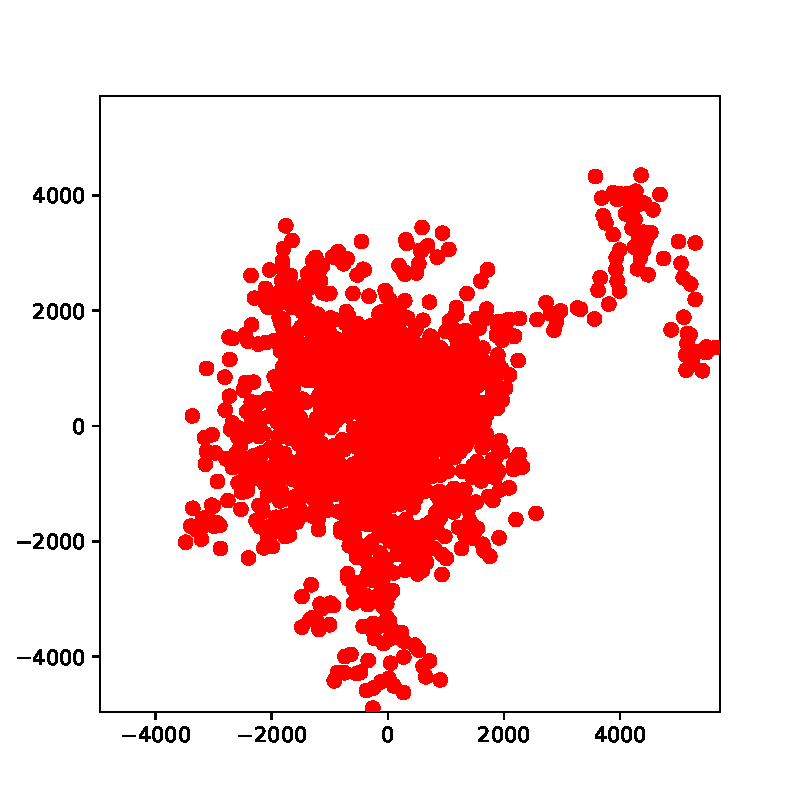
\includegraphics[scale=.5]{cluster_big.pdf}
	

	\end{columns}
	\end{frame}

%------------------------------------------------

\begin{frame}
	\frametitle{(A) Benchmark-Instanzen}
	\begin{columns}[c] % The "c" option specifies centered vertical alignment while the "t" option is used for top vertical alignment
	
	\column{.5\textwidth} % Right column and width
	\textbf{Generiert: Gleichverteilte Punkte}\\
	Erfolgsquote des primitiven Algorithmus
	
	
	\column{.45\textwidth} % Left column and width
	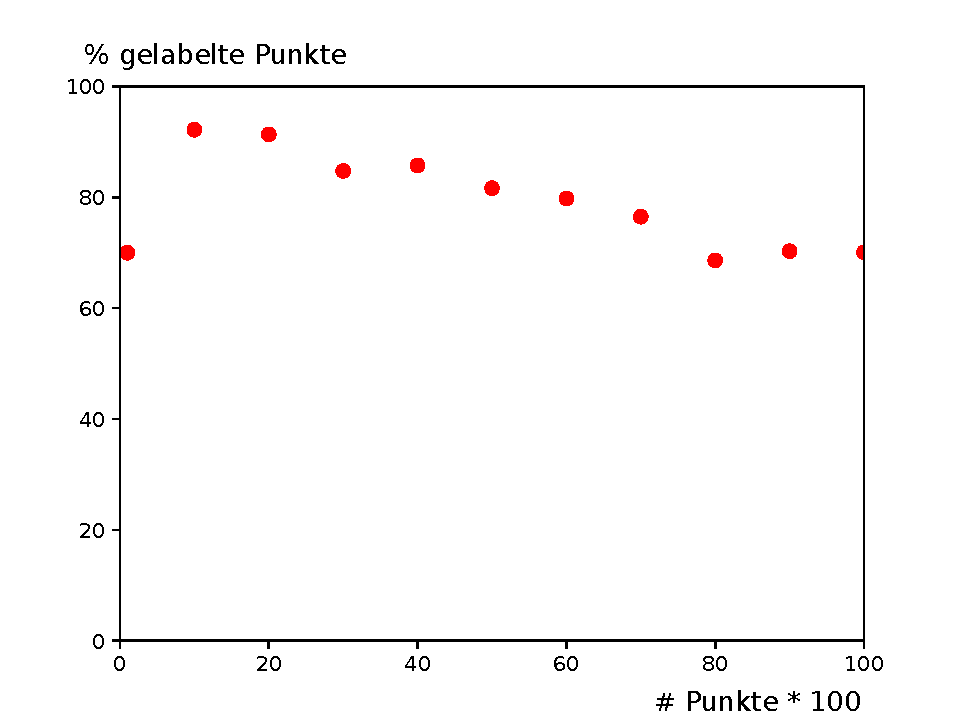
\includegraphics[scale=.45]{cluster_solve.pdf}
	

	\end{columns}
	\end{frame}

%------------------------------------------------


\begin{frame}
	\frametitle{(A) Benchmark-Instanzen}
	\begin{columns}[c] % The "c" option specifies centered vertical alignment while the "t" option is used for top vertical alignment
	
	\column{.5\textwidth} % Right column and width
	\textbf{Geografische Punkte}
	\begin{itemize}
		\item Sehenswürdigkeiten in Berlin: 57\% Erfolgsquote
	\end{itemize}
	
	\column{.45\textwidth} % Left column and width
	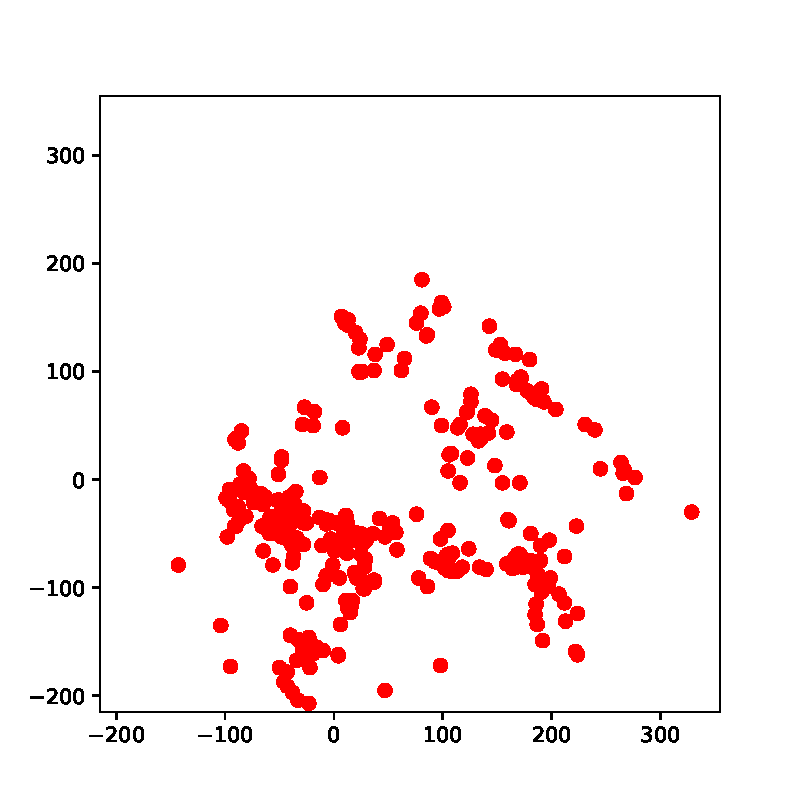
\includegraphics[scale=.5]{tourist.pdf}
	

	\end{columns}
	\end{frame}

%------------------------------------------------


\begin{frame}
	\frametitle{(A) Benchmark-Instanzen}
	\begin{columns}[c] % The "c" option specifies centered vertical alignment while the "t" option is used for top vertical alignment
	
	\column{.5\textwidth} % Right column and width
	\textbf{Geografische Punkte}
	\begin{itemize}
		\item Deutsche Bahnhöfe: 69\% Erfolgsquote
	\end{itemize}
	
	\column{.45\textwidth} % Left column and width
	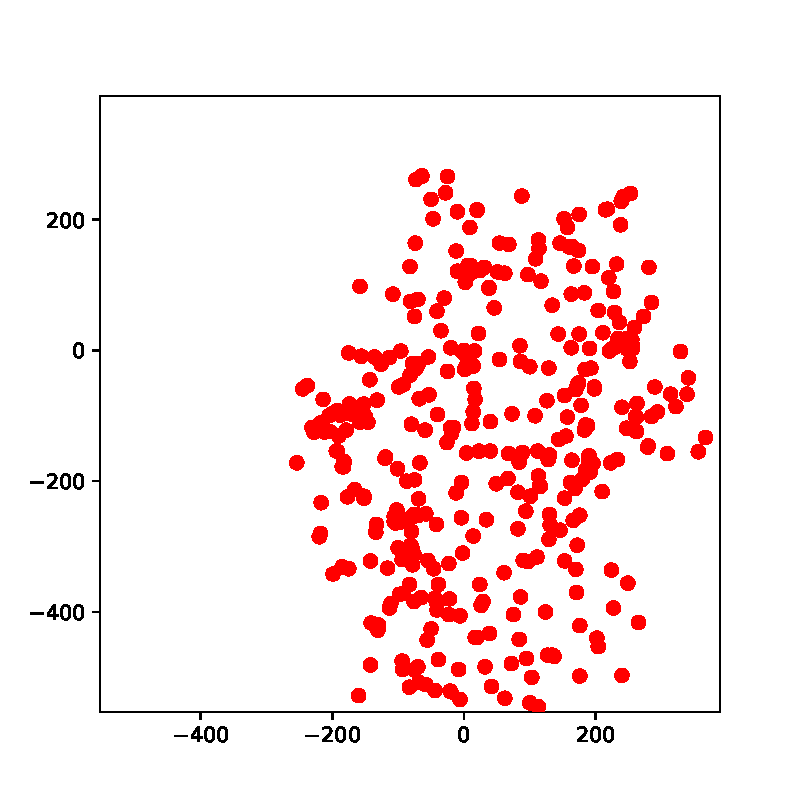
\includegraphics[scale=.5]{railway.pdf}
	

	\end{columns}
	\end{frame}

%------------------------------------------------

\begin{frame}
	\frametitle{(A) Benchmark-Instanzen}
	\begin{columns}[c] % The "c" option specifies centered vertical alignment while the "t" option is used for top vertical alignment
	
	\column{.5\textwidth} % Right column and width
	\textbf{Geografische Punkte}
	\begin{itemize}
		\item US Städte: 68\% Erfolgsquote
	\end{itemize}
	
	\column{.45\textwidth} % Left column and width
	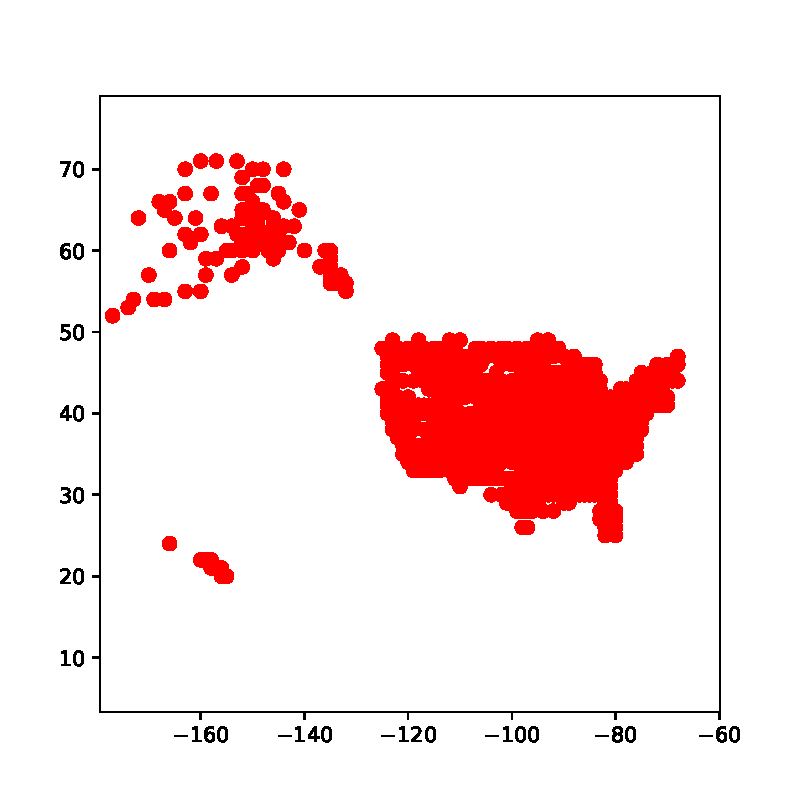
\includegraphics[scale=.5]{cities.pdf}
	

	\end{columns}
	\end{frame}

%------------------------------------------------


\begin{frame}
\frametitle{(B) Algorithmus}
	
\textbf{Greedy Heuristik}
\begin{itemize}
	\item über alle Punkte iterieren
	\item für jeden Punkt alle Labelpositionen ausprobieren
	\item erste Labelposition ohne Konflikt übernehmen
	\item Laufzeit: $\mathcal{O}(n^2)$
\end{itemize}
	

\end{frame}

%------------------------------------------------




\end{document} 